\section{Results}
\label{sec:results}

\subsection{Batch Solver and Extrinsic Pitch}
We use the full-trajectory C++ batch solve as an offline full-batch
reference; offline it reaches
\SI{0.20}{\metre}\,/\,\SI{1.1}{\degree} on slow racing and
\SI{0.64}{\metre}\,/\,\SI{2.5}{\degree} on fast (the dense racing
$\Delta t_p$ over-fits fast racing, where the coarser sliding window
does better).
The radar-to-body pitch is a fixed mount angle, measured at
27--28\degree\ with an inclinometer on the radar face (reference surface
0\degree) and frozen at 27.5\degree, a few degrees below the
30\degree\ \ac{cad} design (3D-printed, hand-assembled fixture).  We lock it
rather than estimate it online because it is only weakly observable from
Doppler: the self-calibration is init-dependent and orientation \ac{rmse} is
pitch-insensitive (\autoref{sec:backflips}).  The batch estimate is
shown for reference (dashed) in the \ac{rpe} curves (\autoref{fig:rpe}).

\subsection{Sliding Window: Settled vs.\ Live}
\label{sec:sw_results}

\autoref{tab:sw} reports sliding window results
(3\,s window, 0.3\,s stride, Schur marginalization).
\autoref{fig:traj} shows trajectory overlays for all three flights;
\autoref{fig:error_time} shows the corresponding error timeseries.

\begin{table}[t]
\centering
\caption{Sliding Window: Settled and Live Leading-Edge \ac{rmse}
  (consistent unscaled prior; per-window solve time on a laptop CPU)}
\label{tab:sw}
\small
\setlength{\tabcolsep}{2.5pt}
\begin{tabular}{@{}llccccc@{}}
\toprule
Bag & Mode & Vel (m/s) & Ori (\degree) & Pos (m) & Drift\% & $t_{\mathrm{win}}$(s) \\
\midrule
\multirow{2}{*}{Slow racing}
  & Settled & 0.42 & 1.53 & 0.293 & 0.61 & \multirow{2}{*}{0.70} \\
  & \textbf{Live edge} & \textbf{0.48} & \textbf{1.97} & \textbf{0.310} & \textbf{0.64} & \\
\midrule
\multirow{2}{*}{Fast racing}
  & Settled & 0.25 & 2.35 & 0.312 & 0.69 & \multirow{2}{*}{0.35} \\
  & \textbf{Live edge} & \textbf{0.32} & \textbf{2.88} & \textbf{0.399} & \textbf{0.88} & \\
\midrule
\multirow{2}{*}{Backflips\textsuperscript{$\ddagger$}}
  & Settled & ---\textsuperscript{$\ast$} & 5.01 & 1.674 & 3.09 & \multirow{2}{*}{0.6} \\
  & \textbf{Live edge} & \textbf{2.35} & \textbf{6.35} & \textbf{1.545} & \textbf{2.85} & \\
\bottomrule
\multicolumn{7}{@{}p{\columnwidth}@{}}{\scriptsize
  All bags use the unscaled consistent marginalization prior
  (\autoref{sec:sw}) and the \emph{same} dynamics-adaptive weighting
  law (\autoref{sec:models}).  Per-regime parameters are limited to
  spline grids ($\Delta t_p{=}5/40/10$\,ms), the heading weight, and
  for backflips the position-init anchor
  ($\lambda_{\mathrm{pos\text{-}init}}{=}0.5$) and flip-regime Doppler
  correction $b{=}{-}1.5$\,m/s (\autoref{sec:backflips}).  Extrinsic
  pitch locked at 27.5\degree\ for all bags.
  $^\ast$Settled velocity is not reported for backflips: stride-boundary
  resampling injects a retrospective-evaluation artifact there.  The live
  column is the deployment-relevant figure throughout.
  Drift\,\%: path lengths 48.1\,m / 44.9\,m / 54.1\,m.
  Iteration-capped configurations reproduce bit-identically across
  repeated runs; full-convergence configurations vary by $<$2\%
  (multithreaded reduction order).}
\end{tabular}
\end{table}

Live-edge orientation degrades 0.4--0.5\degree\ relative to settled;
this is expected because subsequent windows refine previous estimates.
With the consistent prior, settled velocity is smooth across stride
boundaries (the earlier inconsistent prior produced position jumps
that inflated the settled velocity derivative).
We report all tables, plots, and the cross-validation of
\autoref{sec:baselines} at a single \emph{evaluation configuration}
(3\,s window, 0.3\,s stride), chosen for best accuracy and cross-table
consistency rather than as a deployment claim: per-window solve time is set
by window length and knot density, not the stride, and at 3\,s only fast
racing approaches the 0.3\,s budget on a laptop CPU.  Real time is
nonetheless within reach.  Pushing the window and stride to \emph{barely}
reach it per regime costs almost nothing (\autoref{tab:realtime},
\autoref{fig:realtime}): fast is real-time at the 0.3\,s stride with a 2\,s
window, slow and backflips at a 0.5\,s stride (1.5\,s and 2\,s windows),
live accuracy stays within run-to-run noise of the evaluation configuration
(backflips even improves, $6.35\to5.56\degree$), and racing remains under
1\% drift.  Solve times carry $\sim$20\% run-to-run variance, so the strides
are taken with margin.

Deployment, though, asks for more than \emph{barely} real-time.  This
estimator is designed as one factor source in a larger fusion graph
(\autoref{sec:nees}), sharing compute with a parallel visual or lidar
pipeline, so a tuned, no-margin operating point on a dedicated CPU is a
feasibility demonstration, not a deployment budget.  The margin must come
from the back-end: a banded Schur factorization is numerically unstable at
our conditioning, so the route is incremental smoothing, not batch
re-solve.  Girod et al.~\cite{girod2024brio} reach comfortable onboard rates
with exactly such an iSAM2 back-end (on a discrete-time graph); porting our
continuous-time B-spline onto it, where the shared global bias induces a
Bayes-tree fill-in, is the deployment path we leave to future work.
The dominant cost reductions were: the consistent prior removing
the marginalization re-linearization ($\sim$0.6\,s), coarsening
$\Delta t_p$ from 5\,ms to 40\,ms for aggressive flight (which
\emph{also} drops the LM iteration count from 28 to 11 and slightly
improves orientation), and warm-start alignment removing the
live-edge seam.  For a mapping-oriented profile (full iterations,
no warm-start alignment) slow racing settles to 1.14\degree\
orientation (yaw 0.61\degree) at 2.1\,s per window.

\begin{table}[t]
\centering
\caption{\textcolor{red}{[Choose this table \emph{or}
  \autoref{fig:realtime}.] Evaluation configuration (3\,s/0.3\,s, used
  throughout the paper) vs.\ the per-regime real-time point (solve time
  below the stride).  Reaching real time is accuracy-neutral and improves
  backflips.  Live-edge \ac{rmse}; solve times carry $\sim$20\% run-to-run
  variance.}}
\label{tab:realtime}
\small
\setlength{\tabcolsep}{3pt}
\begin{tabular}{@{}llccc@{}}
\toprule
Regime & Win./str.\ (s) & Solve (s) & Live pos (m) & Live ori (\degree) \\
\midrule
\multirow{2}{*}{Fast}
  & 3.0/0.3 (eval.)   & 0.32 & 0.399 & 2.88 \\
  & 2.0/0.3 (real-time) & 0.28 & 0.443 & 2.95 \\
\midrule
\multirow{2}{*}{Slow}
  & 3.0/0.3 (eval.)   & 0.72 & 0.310 & 1.97 \\
  & 1.5/0.5 (real-time) & 0.40 & 0.301 & 1.98 \\
\midrule
\multirow{2}{*}{Backflips}
  & 3.0/0.3 (eval.)   & 0.59 & 1.545 & 6.35 \\
  & 2.0/0.5 (real-time) & 0.43 & \textbf{1.499} & \textbf{5.56} \\
\bottomrule
\end{tabular}
\end{table}

\begin{figure}[t]
  \centering
  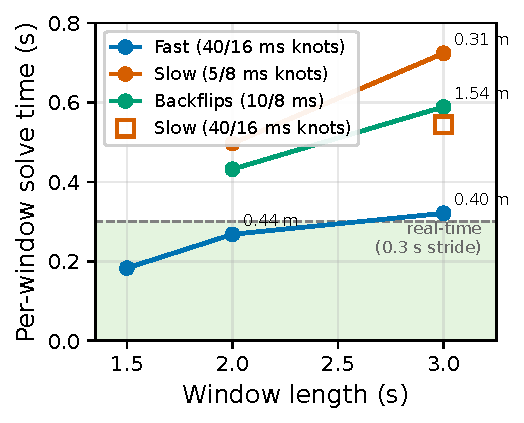
\includegraphics[width=0.86\columnwidth]{figures/realtime_sweep.pdf}
  \caption{\textcolor{red}{[Choose this figure \emph{or}
    \autoref{tab:realtime}.] Per-window solve time vs.\ window length per
    regime; a configuration is real-time when its solve time falls below
    the stride.  Stars mark the per-regime real-time operating point:
    shrinking the window puts fast under a 0.3\,s stride and slow and
    backflips under a 0.5\,s stride, at negligible accuracy cost
    (\autoref{tab:realtime}).  Solve times carry $\sim$20\% variance.}}
  \label{fig:realtime}
\end{figure}

\begin{figure*}[t]
  \centering
  
\includegraphics[width=\textwidth]{figures/traj_combined.pdf}
  \caption{Trajectory overlays for all three flights (columns): \ac{mocap}
    ground truth vs.\ the SW live edge, X--Y (top) and Y--Z (bottom)
    projections; start~$\blacksquare$.  Larger fast-racing deviations
    reflect higher dynamics ($\omega_{\max}=9.1$\,rad/s); on backflips
    the residual ${\sim}6\degree$ live orientation error attenuates the
    loop circles while the donut sweep and altitude are followed.}
  \label{fig:traj}
\end{figure*}

\begin{figure*}[t]
  \centering
  
\includegraphics[width=\textwidth]{figures/error_over_time.pdf}
  \caption{Position, velocity, and orientation error vs.\ time for slow
    racing (top) and fast racing (bottom).  Batch estimate (red dashed)
    and SW live edge (orange dotted).  Fast racing position error
    accumulates monotonically with trajectory length; velocity and
    orientation errors spike at high-speed, high-dynamics sections.}
  \label{fig:error_time}
\end{figure*}

\subsection{Relative Pose Error and Position Drift}
\label{sec:rpe}

\autoref{fig:rpe} shows the KITTI-style translational \ac{rpe} as a
function of segment length for racing bags (batch and SW live) and
backflips (batch only).  At longer segments ($\geq 20$\,m) the global
B-spline smoother reduces error sharply: slow racing batch reaches
\SI{1.08}{\percent} at 20\,m and \SI{1.02}{\percent} at 40\,m; fast
racing stabilises at $\approx$\SI{2.2}{\percent} beyond 20\,m.  At
short segments ($\leq$10\,m) errors are larger (3--8\% for racing)
because the 11\,Hz radar provides only a handful of Doppler
measurements per segment and the global optimizer cannot smooth over
sub-second intervals, a constraint of the radar rate, not a spline
artifact.  Global position drift (\%) remains the headline deployment
metric (live edge); \ac{rpe} is the complementary per-segment view.

\begin{figure}[t]
  \centering
  
\includegraphics[width=\columnwidth]{figures/rpe_drift.pdf}
  \caption{KITTI-style translational \ac{rpe} (end-point displacement error
    as \% of segment length) vs.\ accumulated GT distance.  Left:
    racing bags, batch (solid) and SW live edge (dashed).  Right:
    backflips batch.}
  \label{fig:rpe}
\end{figure}

\subsection{Radar Contribution}
Radar is essential.  Disabling it (\texttt{-{}-no-radar}) collapses the
live-edge estimate to \ac{imu} dead-reckoning: position drift balloons to
5.9\% on slow racing and diverges entirely on fast racing
($\approx$99.5\% of distance, error on the order of the full path
length), with velocity \ac{rmse} rising to 2.4 and
8.0\,m/s as double-integrated accelerometer noise accumulates unbounded.
The direct Doppler velocity constraints bound this to the
\autoref{tab:sw} figures (0.6--0.9\% drift, 0.32--0.48\,m/s velocity),
one-to-two orders of magnitude lower.  Orientation
improves more modestly, from 8.9\degree/4.0\degree\ (\ac{imu}-only) to
2.0\degree/2.9\degree, the 1\,kHz gyroscope already constraining it.

\subsection{Held-Out Validation}
\label{sec:heldout}
All tuning used three bags (slow/fast racing, backflips); the final
configuration was then run \emph{unmodified} on flights never used for
any decision.  A second, independent fast-racing flight reaches
0.37\,m\,/\,2.81\degree\ live (vs.\ 0.40\,m\,/\,2.88\degree\ on the
tuning bag), and a circular trajectory reaches
0.90\,m\,/\,3.77\degree\ live.
Five additional stress-tier bags from an earlier recording day use an
older radar firmware with $12\times$ coarser Doppler quantization
(0.604 vs.\ 0.049\,m/s), partially unusable accelerometer axes, and
per-day time offsets; the default \ac{ransac} prefilter still keeps
$46$--$75\%$ of returns (no starvation), and the system degrades
gracefully (1.5--7\,m position), with the \emph{old-firmware backflips}
orientation reaching 8.1\degree\ settled\,/\,9.1\degree\ live (better
than the 14.8\degree\ of its previous, individually tuned best) under
the untuned universal configuration.  The rate-adaptive weighting thus
transfers across both firmware and day.
A data-health screening (radar frame-rate continuity, \ac{imu}/\ac{mocap}
coverage) precedes all held-out evaluation, since several early bags
contain radar \ac{uart} dropouts; all evaluation windows lie on healthy
spans.  Each flight condition is a single representative recording; the
evaluation's breadth comes from these held-out flights and the
cross-platform validation of \autoref{sec:baselines} rather than
repeated trials (\autoref{sec:stat_scope}).

\subsection{External Cross-Validation Against EKF Baselines}
\label{sec:baselines}
We cross-validate against the \ac{ekf}-\ac{rio} family of Doer and
Trommer~\cite{doer2020ekf,doer2021yrio} in both directions on shared
data, with their toolbox pinned at a fixed commit and every parameter
deviation documented in the repository.

\textbf{Our system on their data.}  We run our sliding-window solver,
with the universal weighting configuration unmodified, on the four
public ICINS-2021 indoor flight datasets~\cite{doer2021yrio}
(TI IWR6843AOP at 10\,Hz, Analog Devices ADIS16448 \ac{imu} at 409\,Hz with
onboard barometer, loop-closure-and-scale-corrected VINS pseudo ground
truth), using their published extrinsic calibration (locked) and
their $\pm 60\degree$ elevation pre-gate.  Their estimators
(\mbox{ekf-rio}, unaided yaw; \mbox{ekf-yrio}, Manhattan-world radar
yaw aiding) are re-run from their stock configurations on the same
bags, and \emph{both} systems are evaluated with the identical causal
protocol of \autoref{sec:setup} (live estimates, start-anchored
alignment, same windows and ground truth).
\autoref{tab:baselines} reports the headline metrics~(a) and their
decomposition~(b).  On position our
solver reaches the same order of magnitude as the baselines (0.5--1.9\,m,
0.6--1.3\% drift).  It trails the yaw-aided ekf-yrio on absolute
position (best on all four flights), but velocity \ac{rmse}
0.07--0.08\,m/s matches theirs and the order-of-magnitude vertical gap
closes (below).
The full 3-DoF orientation column favors our solver
(0.51--1.13\degree\ vs.\ up to $10.1\degree$), but this gap is almost
entirely \emph{yaw}: our heading is anchored by a pseudo-magnetometer
(here the VINS pseudo-GT yaw used as a magnetometer surrogate, in
place of the \ac{mocap} yaw available on our own platform), whereas
ekf-yrio uses sensor-only Manhattan-world yaw and ekf-rio is unaided.
On the heading-\emph{independent} roll and pitch the three systems are
comparable ($0.25$--$0.74\degree$, \autoref{tab:baselines}(b)),
so the orientation column is not an attitude win; removing our heading
aiding confirms this: on flight\_1 our unaided yaw drifts to
$9.9\degree$, matching unaided ekf-rio ($10.1\degree$), while roll/pitch
and position are essentially unchanged.

The default \ac{ransac} prefilter (\autoref{sec:models}) buys this
same-order position, its clearest single demonstration.
A single-chip 2-TX array has limited
elevation diversity, and a minority of returns carry an
elevation-correlated Doppler bias.  Doer's \mbox{reve} rejects these
with 3D \ac{ransac} (inlier $0.15$\,m/s); a Huber-robust least squares only
down-weights them.  Measured against the ground-truth attitude, the
per-frame vertical ego-velocity bias is $-0.06$ to $-0.16$\,m/s under a
Huber-only front-end but at most $0.10$\,m/s in magnitude under \ac{ransac}.
With the prefilter \emph{disabled}, our vertical channel accumulates a
large systematic error (whole-trajectory \ac{ate} $9.6$\,m on flight\_1,
$12$--$15\%$ vertical drift) that the baselines do not exhibit (theirs
stays $\sim$0.2--0.3\,m); the \ac{ransac} prefilter removes it
at the source on all four flights, cutting whole-trajectory \ac{ate} to
$0.24$--$0.76$\,m (\autoref{tab:baselines}(b)) and bringing
position back into the baselines' range.  Their vertical accuracy is
not altitude aiding either: disabling the barometer in ekf-yrio shifts
its vertical drift by $\le$0.04\,m (stock $\sigma_\mathrm{altimeter}{=}5$\,m
makes it near-negligible), so they too estimate vertical from radar and
\ac{imu} alone, by the same outlier-rejection mechanism.  The single-chip
elevation bias is therefore real but not fundamental: an
outlier-rejection gap, closed by the same \ac{ransac} stage the
baselines use.  Under
whole-trajectory Umeyama alignment (\autoref{tab:baselines}(b))
all three systems agree to $\le$1\,m, consistent with the baselines'
published full-alignment figures (they are faithfully reproduced) and
confirming that our default front-end matches them.

\textbf{Their filters on our data.}  The reverse port is a
\emph{sensor/stack-coupling characterization}, not a head-to-head
comparison; it is regime-dependent, and we report the measured
outcome rather than a verdict.  Here we port ekf-rio and its multi-radar generalization
x-rio~\cite{doer2021xrio} (run single-radar); ekf-yrio, the yaw-aided
single-radar variant Doer benchmarks the ICINS flights with, was the
forward-port comparator above.  On the slow-racing flight both ekf-rio
and x-rio fail: their
$\chi^2(3)$ innovation gate rejects $99.7\%$ of the radar ego-velocity
updates (301 of 302), so the filter reverts to \ac{imu} dead-reckoning and
runs essentially unconstrained ($>2$\,km of error for both, almost
entirely vertical, $\approx\tfrac12 g t^2$).  On the faster flight ekf-rio
instead survives, degrading to $1.4$\,m ($3.1\%$ drift,
$9.0\degree$): its larger translational excitation produces radar
ego-velocities that clear the gate (only $64\%$ rejected), enough to
constrain the filter.  The amount of radar information admitted thus
scales with how strongly motion excites the sparse Doppler, and the
common cause is a stack-level mismatch rather than a defect of their
method: our best-velocity firmware yields only $\sim$13 points per
frame (their \ac{ransac}/$\sigma$-gates expect hundreds, and ego-velocity
estimation fails outright on roughly half of all scans), there is no
hardware radar trigger, and our racing-frame vibration (measured gyro
white-noise PSD $2.1\degree/\mathrm{s}/\sqrt{\mathrm{Hz}}$ in flight)
exceeds their process-noise parameter range, making propagation
overconfident so the gate then rejects the few updates that survive.
This is a design-space split (\autoref{sec:conclusion}), not a defect of
either method: their stack runs near sensor rate on dense clouds, ours
spends \SI{0.35}{}--\SI{0.70}{\second} per window on sparse Doppler,
an accuracy-versus-latency trade.

\begin{table*}[t]
\caption{Cross-validation on the public ICINS-2021 flight
datasets~\cite{doer2021yrio}, all systems under our causal protocol
(live estimate, start-anchored alignment).
\textbf{(a)}~Headline metrics; heading aiding differs by design (see text).
\textbf{(b)}~Decomposition, making the honest structure visible at a
glance: \emph{roll/pitch} is the heading-independent attitude \ac{rmse}
(per-axis RMS, yaw excluded), so the large orientation gap in~(a) is yaw,
not attitude; \emph{our drift} splits our position error into horizontal
and vertical, both sub-1.3\% under the default \ac{ransac} prefilter
(\autoref{sec:models}; the footnote gives the prefilter-disabled figures
for contrast); \emph{whole-traj.\ \ac{ate}} re-evaluates every system under the
standard EVO/KITTI Umeyama alignment (no scale) for cross-checking against
published figures.}
\label{tab:baselines}
\centering
\footnotesize
% Box both subtables, then centre each within the wider one's width so they
% share one axis; footnote kept out of the tabular so it cannot stretch the
% last column.
\setlength{\tabcolsep}{6pt}%
\sbox0{\begin{tabular}{lccc}
\toprule
\multicolumn{4}{l}{\textit{(a)~Headline: position [m] / velocity [m/s] / orientation [\degree] / drift [\%]}}\\
\midrule
Flight (path) & ekf-rio & ekf-yrio & Ours \\
\midrule
1 (142\,m) & 1.41 / 0.20 / 10.1 / 1.0 & \textbf{0.39} / \textbf{0.08} / 0.70 / \textbf{0.3} & 0.92 / 0.08 / \textbf{0.51} / 0.6 \\
2 (45\,m)  & 0.25 / 0.08 / 1.59 / 0.6 & \textbf{0.20} / \textbf{0.08} / \textbf{0.91} / \textbf{0.4} & 0.51 / 0.08 / 0.94 / 1.1 \\
3 (147\,m) & \textbf{0.47} / 0.08 / 1.07 / \textbf{0.3} & 0.48 / 0.08 / 1.09 / \textbf{0.3} & 1.92 / \textbf{0.07} / \textbf{0.52} / 1.3 \\
4 (78\,m)  & 0.39 / 0.09 / 3.67 / 0.5 & \textbf{0.22} / \textbf{0.07} / 1.41 / \textbf{0.3} & 0.92 / 0.07 / \textbf{1.13} / 1.2 \\
\bottomrule
\end{tabular}}%
\setlength{\tabcolsep}{5pt}%
\sbox2{\begin{tabular}{lcccccccc}
\toprule
\multicolumn{9}{l}{\textit{(b)~Decomposition}}\\
\midrule
 & \multicolumn{3}{c}{Roll/pitch \ac{rmse} [\degree]} & \multicolumn{2}{c}{Our drift [\% path]} & \multicolumn{3}{c}{Whole-traj.\ \ac{ate} [m]} \\
\cmidrule(lr){2-4}\cmidrule(lr){5-6}\cmidrule(lr){7-9}
Flight & ekf-rio & ekf-yrio & Ours & horiz.\ & vert.\ & ekf-rio & ekf-yrio & Ours \\
\midrule
1 & 0.24 & 0.25 & 0.25 & 0.16 & 0.63 & 0.87 & 0.23 & 0.46 \\
2 & 0.57 & 0.59 & 0.55 & 0.14 & 1.13 & 0.13 & 0.10 & 0.24 \\
3 & 0.25 & 0.26 & 0.27 & 0.30 & 1.28 & 0.36 & 0.26 & 0.76 \\
4 & 0.74 & 0.74 & 0.74 & 0.26 & 1.15 & 0.30 & 0.15 & 0.46 \\
\bottomrule
\end{tabular}}%
\dimen0=\wd0 \ifdim\wd2>\dimen0 \dimen0=\wd2 \fi
\makebox[\dimen0][c]{\usebox0}

\vspace{5pt}

\makebox[\dimen0][c]{\usebox2}

\vspace{2pt}

\parbox{\dimen0}{\raggedright\footnotesize Prefilter \emph{disabled} (Huber-only): our vertical drift $12$--$15\%$; whole-traj.\ \ac{ate} $9.57/2.88/10.86/5.48$\,m (flights~1--4).\par}
\end{table*}

\subsection{Output Covariance Consistency (NEES)}
\label{sec:nees}
A factor source for a larger fusion graph must report \emph{honest}
covariance.  We extract the live-edge joint covariance of
$(\vv_w, \vR)$ each window from the converged problem
(\texttt{ceres::Covariance} over the active support control points,
tangent space, marginalization prior included) and compute the
normalized estimation error squared (\ac{nees}) against \ac{mocap};
for a consistent estimator the \ac{nees} of each 3-DoF block is
$\chi^2_3$-distributed with mean~3.
On the racing flights, summarized by the per-window median for
\emph{both} channels, the \emph{orientation} \ac{nees} is $1.2$--$2.6$
and the velocity \ac{nees} $1.4$--$5.4$ (consistent value~3):
orientation is essentially calibrated (slightly conservative on slow
racing, near-exact on fast, as the weights approximate effective-noise
whitening), and velocity is calibrated to mildly overconfident.  We
report the median, not the mean, because the means (velocity especially)
are inflated by a few windows where the finite-difference \ac{mocap}
velocity reference is unreliable.  Both are \emph{calibration checks}, not powered
hypothesis tests: consecutive windows are temporally correlated, so the
$\chi^2_3$ mean-3 expectation holds only heuristically.  On backflips the
orientation covariance is overconfident
by ${\sim}3\times$ in standard deviation (unmodeled flip-time error) and
only 6 of 50 windows survive the ground-truth quality mask
(\autoref{sec:setup}), too few to support a consistency statement, so
we report it as a caveat rather than a result.  Deployment recipe: inflate the emitted covariance per
regime ($1\times$ gentle, $3\times$ aggressive), or calibrate online
from innovations.

\subsection{Ablation Studies}
\autoref{tab:ablations} summarizes key design choices.

\begin{table}[t]
\centering
\caption{Selected Ablation Results (batch solver, slow\_racing unless noted)}
\label{tab:ablations}
\small
\setlength{\tabcolsep}{4pt}
\begin{tabular}{@{}lcc@{}}
\toprule
Configuration & Pos (m) & Ori (\degree) \\
\midrule
\multicolumn{3}{l}{\textit{\ac{imu} rate (slow\_racing batch, no lever arm\textsuperscript{\dag})}} \\
\quad 200\,Hz & 0.525 & 1.64 \\
\quad \textbf{1000\,Hz (default)} & \textbf{0.183} & \textbf{1.02} \\
\midrule
\multicolumn{3}{l}{\textit{Lever-arm correction $\boldsymbol{\omega}{\times}\mathbf{t}_{bs}$ (batch)}} \\
\quad No correction --- slow racing   & 0.183 & 1.02 \\
\quad\quad\quad\quad\quad\ --- fast racing   & 0.862 & 2.73 \\
\quad\quad\quad\quad\quad\ --- backflips     & 1.814 & 8.64 \\
\quad \textbf{With correction --- slow}     & \textbf{0.169}  & \textbf{1.02} \\
\quad\quad\quad\quad\quad\quad\ \textbf{--- fast}     & \textbf{0.768}  & \textbf{2.64} \\
\quad\quad\quad\quad\quad\quad\ \textbf{--- backflips} & \textbf{1.814} & \textbf{8.44} \\
\midrule
\multicolumn{3}{l}{\textit{\ac{imu} preintegration vs.\ raw factors (slow\_racing batch)}} \\
\quad Forster TRO-2017 preint.\ at 100\,Hz & 0.288 & 6.40 \\
\quad \textbf{Raw gyro/accel at 1\,kHz (default)} & \textbf{0.169} & \textbf{1.02} \\
\midrule
\multicolumn{3}{l}{\textit{Orientation regularization (backflips batch)}} \\
\quad Min-$\omega$ ($\lambda_{\omega}{=}0.001$) & 1.816 & 8.62 \\
\quad \textbf{Min-$\alpha$, $\lambda_\alpha{=}0.1$ (default)} & \textbf{1.814} & \textbf{8.44} \\
\quad Min-$\alpha$, $\lambda_\alpha{=}1.0$ & 2.069 & 83.8 \\
\midrule
\multicolumn{3}{l}{\textit{SW window dur.\ (slow\_racing SW, settled / live edge)}} \\
\quad 1.5\,s & 0.292 / 0.299 & 1.51 / 2.01 \\
\quad \textbf{3.0\,s (default)} & \textbf{0.293 / 0.310} & \textbf{1.53 / 1.97} \\
\quad 5.0\,s & 0.313 / 0.341 & 1.49 / 2.03 \\
\midrule
\multicolumn{3}{l}{\textit{SW window dur.\ (fast\_racing SW, settled / live edge)}} \\
\quad 2.0\,s & 0.380 / 0.443 & 2.31 / 2.95 \\
\quad \textbf{3.0\,s (default)} & \textbf{0.312 / 0.399} & \textbf{2.35 / 2.88} \\
\midrule
\multicolumn{3}{l}{\textit{Marginalization (fast\_racing SW, settled)}\textsuperscript{\ddag}} \\
\quad None (boundary prior only) & 0.412 & 2.71 \\
\quad \textbf{Schur complement} & \textbf{0.312} & \textbf{2.35} \\
\midrule
\multicolumn{3}{l}{\textit{Extrinsic optimization (slow\_racing batch)}\textsuperscript{\S}} \\
\quad \textbf{Pitch $\delta$ optimized (default)} & \textbf{0.169} & \textbf{1.02} \\
\quad Pitch $\delta$ locked & 0.157 & 1.02 \\
\bottomrule
\multicolumn{3}{@{}p{\columnwidth}@{}}{\scriptsize
  Batch rows (\ac{imu}-rate, lever-arm, ori-reg, extrinsic) isolate one
  design choice at a fixed pre-\ac{ransac} operating point; the \ac{ransac} default
  shifts batch absolutes (slow batch 0.169$\to$0.198\,m, fast
  0.768$\to$0.64\,m, the \autoref{sec:results} batch figures) without
  changing orderings.  The SW rows (window duration, marginalization)
  are under the \ac{ransac} default.  All runs use the sensor-only init
  (\autoref{sec:init}); the bias seed shifts batch absolutes comparably,
  again without changing orderings.
  \textsuperscript{\dag}Lever arm disabled for isolation; see Lever-arm rows
  for the current default (0.169\,m/1.02\degree).
  \textsuperscript{\ddag}Marginalization shown for \texttt{fast\_racing}; on
  slow\_racing the near-zero optimal prior makes Schur and boundary-only
  nearly equivalent.
  \textsuperscript{\S}C++ solver supports only 1-DoF pitch offset (roll/yaw
  unobservable from Doppler; free 3-angle optimization tested in Python
  solver showed 6--8\degree\ orientation runaway; see
  \autoref{sec:negative}).}\\
\end{tabular}
\end{table}

\textbf{Key observations from \autoref{tab:ablations}.}
Full-rate \ac{imu} (1\,kHz) improves position by $2.9\times$ over 200\,Hz,
motivating the tight bias priors in \texttt{solver\_cpp.yaml}.
Lever-arm correction helps racing ($8$--$11\%$ position) but has
negligible effect on backflips: at $\Delta t_o{=}0.8$\,ms the dense
spline absorbs the $|\bm{\omega}{\times}\mathbf{t}_{bs}|\approx1$\,m/s
term through orientation DoF.
Schur marginalization reduces fast-racing settled position by 24\%
(0.412\,m $\to$ 0.312\,m); for slow racing the optimal prior scale is
$10^{-7}$ (near-zero), so both variants give equivalent results;
the benefit is captured in \autoref{tab:prior_scale} instead.
Window duration has little effect on either racing regime: slow stays at
live 0.30--0.34\,m across 1.5--5\,s, and fast gives essentially equal
orientation at 2\,s and 3\,s (settled 2.31\degree\ vs 2.35\degree) with
3\,s modestly better on position (live drift 0.98 vs 0.88\%).  We keep
3\,s as the default for that small position gain, trading latency.
We lock pitch at its measured value for all sliding-window runs; even
in the batch ablation, locking is marginally better than freeing it
(0.157 vs.\ 0.169\,m on slow racing), consistent with the pitch being
only weakly observable (\autoref{sec:backflips}).
